\section{Radii\-Ellipse Class Reference}
\label{classRadiiEllipse}\index{RadiiEllipse@{RadiiEllipse}}
{\tt \#include $<$radiiellipse.h$>$}

Inheritance diagram for Radii\-Ellipse::\begin{figure}[H]
\begin{center}
\leavevmode
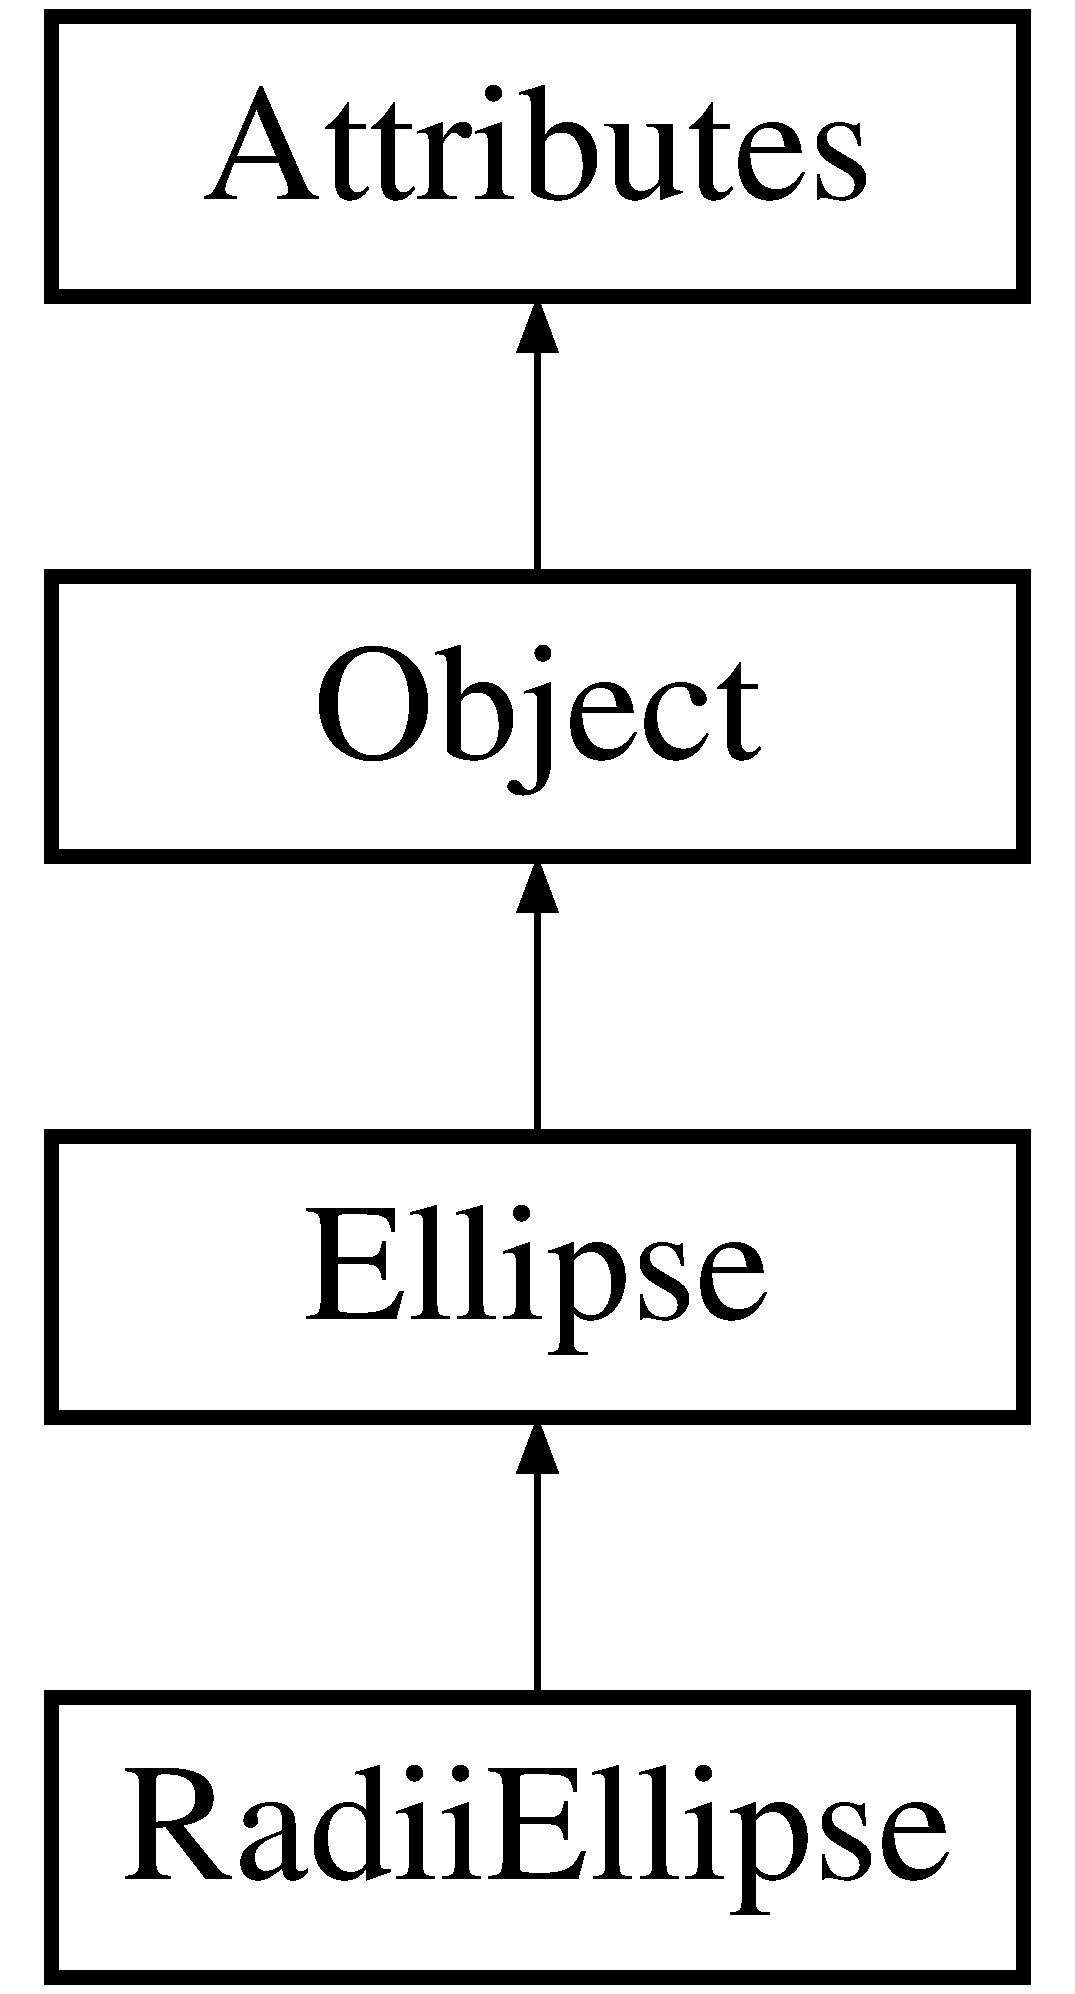
\includegraphics[height=4cm]{classRadiiEllipse}
\end{center}
\end{figure}
\subsection*{Public Methods}
\begin{CompactItemize}
\item 
{\bf Radii\-Ellipse} ()
\item 
{\bf Radii\-Ellipse} ({\bf Coordinate} $\ast$, {\bf Coordinate} $\ast$)
\item 
{\bf $\sim$Radii\-Ellipse} ()
\end{CompactItemize}


\subsection{Detailed Description}
This class handles ellipses defined by their center and radii. This class is derived from {\bf Ellipse} {\rm (p.\,\pageref{classEllipse})}. \begin{Desc}
\item[Author: ]\par
Anthony Liekens \end{Desc}




\subsection{Constructor \& Destructor Documentation}
\index{RadiiEllipse@{Radii\-Ellipse}!RadiiEllipse@{RadiiEllipse}}
\index{RadiiEllipse@{RadiiEllipse}!RadiiEllipse@{Radii\-Ellipse}}
\subsubsection{\setlength{\rightskip}{0pt plus 5cm}Radii\-Ellipse::Radii\-Ellipse ()}\label{classRadiiEllipse_a0}


\index{RadiiEllipse@{Radii\-Ellipse}!RadiiEllipse@{RadiiEllipse}}
\index{RadiiEllipse@{RadiiEllipse}!RadiiEllipse@{Radii\-Ellipse}}
\subsubsection{\setlength{\rightskip}{0pt plus 5cm}Radii\-Ellipse::Radii\-Ellipse ({\bf Coordinate} $\ast$, {\bf Coordinate} $\ast$)}\label{classRadiiEllipse_a1}


\index{RadiiEllipse@{Radii\-Ellipse}!~RadiiEllipse@{$\sim$RadiiEllipse}}
\index{~RadiiEllipse@{$\sim$RadiiEllipse}!RadiiEllipse@{Radii\-Ellipse}}
\subsubsection{\setlength{\rightskip}{0pt plus 5cm}Radii\-Ellipse::$\sim$Radii\-Ellipse ()}\label{classRadiiEllipse_a2}




The documentation for this class was generated from the following files:\begin{CompactItemize}
\item 
{\bf radiiellipse.h}\item 
{\bf radiiellipse.cpp}\end{CompactItemize}
